\documentclass[12pt]{mwart}
\usepackage{polski}
\usepackage[utf8]{inputenc}
\usepackage[T1]{fontenc}
\usepackage{lmodern}
\usepackage{mathtools,amsthm,amssymb,icomma,upgreek,xfrac,enumitem,multicol,paracol,amsmath}
%\usepackage[hidelinks,breaklinks,pdfusetitle,pdfdisplaydoctitle]{hyperref}
\usepackage{cancel}
\mathtoolsset{showonlyrefs,mathic}
\title{\textbf{Raport 1.}}
\author{\fontsize{12pt}{12pt}\selectfont \emph{Klaudia Janicka, 262268}}
\date{10 maja 2022}
\usepackage{float,hyperref}
\usepackage{extsizes}
\usepackage[margin=0.3in]{geometry}

%\setlist[enumerate]{}
\setlist[itemize]{itemsep=0.3em}

\DeclareMathOperator{\diff}{d\!}

\begin{document}
	\maketitle
	\section{Informacje}
	\noindent Dane pochodzą ze strony finance.yahoo.com. Zbiory danych to odpowiednio: X - kurs funta brytyjskiego w przeliczeniu na dolary (GBP/USD), Y - kurs euro w przeliczeniu na dolary (EUR/USD). Do analizy użyto dziennych danych z okresu 5 lat, od 17 kwietnia 2017 roku do 17 kwietnia 2022 roku. Ze zbiorów zostały usunięte wiersze z brakiem danych. Ostateczna liczba wierszy obu zbiorów wynosi 1303.
	\section{Analiza}
	\noindent Wszystkie statystyki zostały obliczone za pomocą własnoręcznie napisanych programów z użyciem estymatorów nieobciążonych lub funkcji wbudowanych.
	\begin{table}[H]
		\centering
		\begin{tabular}{|l|l|l|} 
			\hline
			\phantom{a} & $X$&$Y$ \\ \hline
			\text{Mediana} & 1.3120 & 1.1532 \\ \hline
			\text{Kwartyl rzędu $\frac{1}{4}$} & 1.2866 & 1.1207 \\ \hline
			\text{Kwartyl rzędu $\frac{3}{4}$} & 1.3558 & 1.1842 \\ \hline
			\text{Rozstęp międzykwartylowy} & 0.0691 & 0.0635 \\ \hline
			\text{Rozstęp} & 0.2845  &0.1901 \\ \hline
			\text{Wariancja} & 0.0026 &0.0017 \\ \hline
			\text{Odchylenie standardowe} & 0.0507&0.0415 \\ \hline
			\text{Współczynnik zmienności} & 3.85\% & 3.60\% \\ \hline
		\end{tabular}
	\caption{Tabela charakterystyk zbiorów X i Y}
	\end{table}
\noindent Mediana to wartość, powyżej i poniżej której znajduje się jednakowa liczba obserwacji. Kwantyle spełniają relację $F(x_p) = p$, gdzie $p$ to wartość kwantyla, która nas interesuje. Rozstęp międzykwartylowy to różnica między kwartylami rzędów $\frac{1}{4}$ oraz $\frac{3}{4}.$ Rozstęp jest różnicą między wartością największą i najmniejszą zbioru. Wariancję obliczamy ze wzoru: $\sigma^2 = \frac{1}{n-1}\sum\limits_{i=1}^{n}(x_i-\overline{x})^2$. Jest to estymator nieobciążony. Odchylenie standardowe to pierwiastek kwadratowy z wariancji. Współczynnik zmienności to parametr określający miarę zróżnicowania cechy. \\
Niektóre z charakterystyk obu zbiorów są do siebie dość zbliżone, np. współczynniki zmienności w obu zbiorach różnią się od siebie o $0,25\%$. 
	%scaterplot
	\begin{figure}[H]
		\begin{minipage}{.5\linewidth}
			\centering
			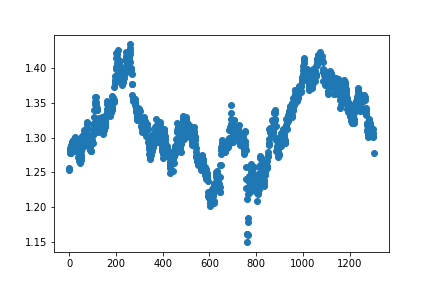
\includegraphics[scale=0.7]{X_sc.PNG}
			\caption{Scatterplot zbioru X}
		\end{minipage}
		$\quad$
		\begin{minipage}{.5\linewidth}
			\centering
			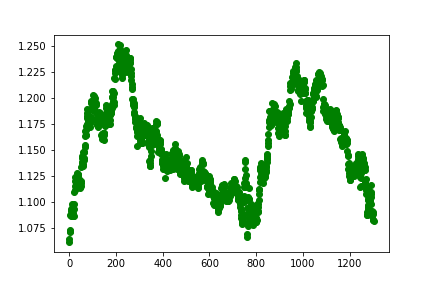
\includegraphics[scale=0.7]{Y_sc.PNG}
			\caption{Scatterplot zbioru Y}
		\end{minipage}
	\end{figure}
\noindent Scatterploty zbiorów wykonano w celu zobrazowania jak przebiegały obniżki i wzrosty kursów EUR i GBP. Oś $x$ reprezentują kolejne liczby porządkowe danych. 
	\section{Interpretacja}
	\begin{table}[H]
		\centering
		\begin{tabular}{|l|l|l|} 
			\hline
			\text{Średnia} & $X$&$Y$ \\ \hline
			\text{Arytmetyczna} & 1.3177 & 1.1541 \\ \hline
			\text{Geometryczna} & 1.3167 & 1.1537 \\ \hline
			\text{Harmoniczna} & 1.3157  &1.1526 \\ \hline
		\end{tabular}
	\caption{Tabela średnich arytmetycznych, geometrycznych i harmonicznych dla zbiorów X i Y}
	\end{table}
\noindent Obliczone wartości kolejnych średnich zostały zaokrąglone do czterech miejsc po przecinku w celu zaprezentowania nieznacznych różnic między nimi. Średnią arytmetyczną obliczamy ze wzoru:
\begin{equation}
	\overline{x_a} = \frac{1}{n}\sum\limits_{i=1}^{n} x_i
\end{equation}
Średnią geometryczną obliczamy ze wzoru:
\begin{equation}
\overline{x_g}=\sqrt[n]{x_1\cdot x_2\cdot \ldots \cdot x_n}
\end{equation}
Średnią harmoniczną obliczamy ze wzoru:
\begin{equation}
	\overline{x_h} = \cfrac{n}{\sum\limits_{i=1}^{n} \frac{1}{x_i}}
\end{equation}
%Hist
\begin{figure}[H]
	\begin{minipage}{.5\linewidth}
		\centering
		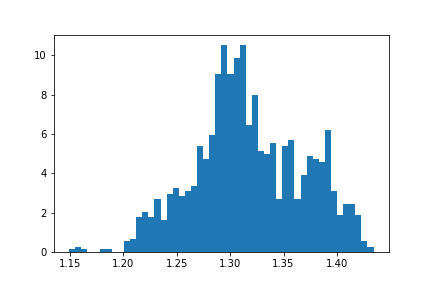
\includegraphics[scale=0.7]{X_hist.PNG}
		\caption{Histogram zbioru X}
	\end{minipage}
	$\quad$
	\begin{minipage}{.5\linewidth}
		\centering
		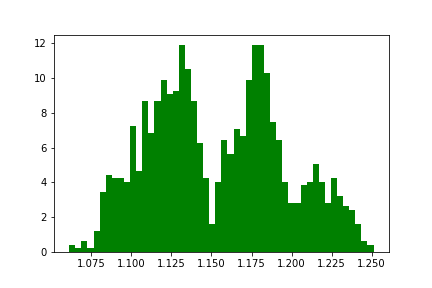
\includegraphics[scale=0.7]{Y_hist.PNG}
		\caption{Histogram zbioru Y}
	\end{minipage}
\end{figure}
Histogramy zbiorów X i Y pokazują liczbę obserwacji poszczególnych wartości kursu. W zbiorze X najczęściej występują wartości ze środka zbioru, z zakresu $1,27-1,33$. Natomiast w zbiorze Y, inaczej niż w przypadku X, mamy dwa najczęściej występujące zakresy: $1,12-13,5$ oraz $1,17-1,185$. Oczywiście są to przybliżone zakresy, odczytane na podstawie wykresu.
%Gęstość
\begin{figure}[H]
	\begin{minipage}{.5\linewidth}
		\centering
		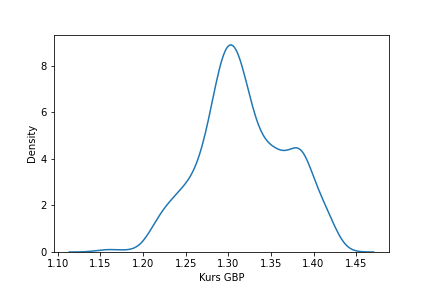
\includegraphics[scale=0.7]{X_kde.PNG}
		\caption{Gęstość zbioru X}
	\end{minipage}
	$\quad$
	\begin{minipage}{.5\linewidth}
		\centering
		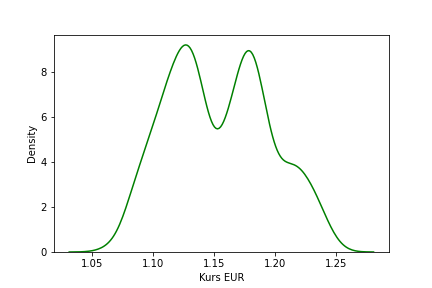
\includegraphics[scale=0.7]{Y_kde.PNG}
		\caption{Gęstość zbioru Y}
	\end{minipage}
\end{figure}
\noindent Gęstości to wygładzone histogramy i reprezentuje dokładnie to samo za pomocą ciągłej funkcji zamiast słupków. Jak widzimy nie zawierają wszystkich słupków przedstawionych na histogramie. W przypadku zbioru Y linia gęstości nie schodzi w pewnym momencie do odpowiedniego poziomu występowania obserwacji.
%Dystrybuanta
\begin{figure}[H]
	\begin{minipage}{.5\linewidth}
		\centering
		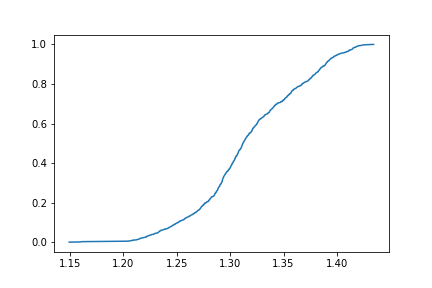
\includegraphics[scale=0.7]{X_cdf.PNG}
		\caption{Dystrybuanta zbioru X}
	\end{minipage}
	$\quad$
	\begin{minipage}{.5\linewidth}
		\centering
		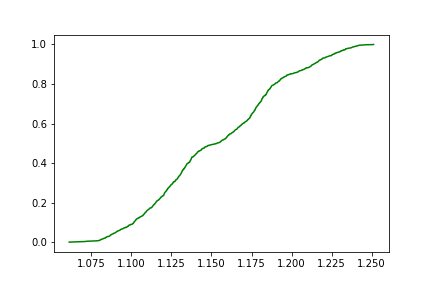
\includegraphics[scale=0.7]{Y_cdf.PNG}
		\caption{Dystrybuanta zbioru Y}
	\end{minipage}
\end{figure}
\noindent Dystrybuanta informuje nas o prawdopodobieństwie wystąpienia wartości mniejszych bądź mniejszych od tej, która nas interesuje $P(Z \leq t)$. I tak na przykład szansa, że ze zbioru X otrzymamy wartość $\leq 1,25$ wynosi $\sim 0.1$, w zbiorze Y szansa na otrzymanie tej samej wartości wynosi już $1$.
%Średnie ucinane
\begin{figure}[H]
	\begin{minipage}{.5\linewidth}
		\centering
		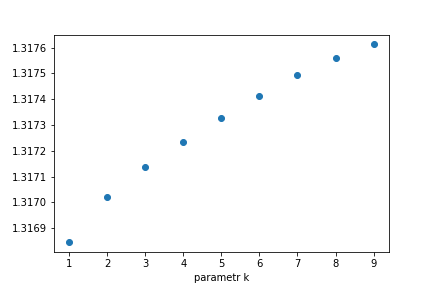
\includegraphics[scale=0.7]{X_trim.PNG}
		\caption{Średnia ucinana zbioru X w zależności od parametru k}
	\end{minipage}
	$\quad$
	\begin{minipage}{.5\linewidth}
		\centering
		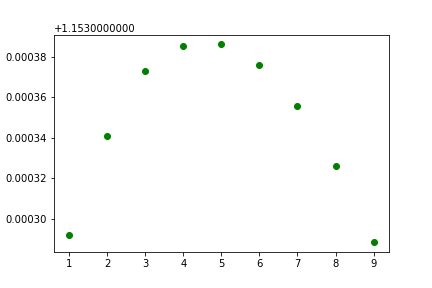
\includegraphics[scale=0.7]{Y_trim.PNG}
		\caption{Średnia ucinana zbioru Y w zależności od parametru k}
	\end{minipage}
\end{figure}
\noindent Średnią ucinaną obliczamy ze wzoru: 
\begin{equation}
	\overline{x_{tk}} = \frac{1}{n-2k}\sum\limits_{i=k+1}^{n-k} x_i
\end{equation}
Średnia ucinana zbioru X w zależności od parametru k wzrasta liniowo, natomiast Y - krzywoliniowo.
%średnie winsorowskie
\begin{figure}[H]
	\begin{minipage}{.5\linewidth}
		\centering
		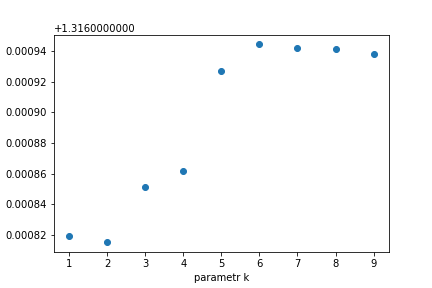
\includegraphics[scale=0.7]{X_wins.PNG}
		\caption{Średnia winsorowska zbioru X w zależności od parametru k}
	\end{minipage}
	$\quad$
	\begin{minipage}{.5\linewidth}
		\centering
		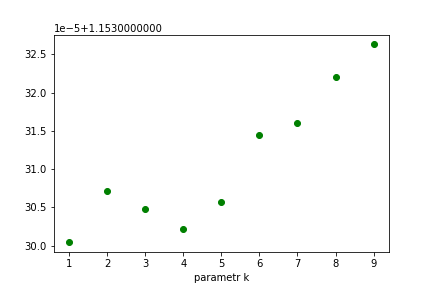
\includegraphics[scale=0.7]{Y_wins.PNG}
		\caption{Średnia winsorowska zbioru Y w zależności od parametru k}
	\end{minipage}
\end{figure}
Średnią winsorowską obliczamy ze wzoru: 
\begin{equation}
	\overline{x_{wk}} = \frac{1}{n}\left[(k+1)x_{k+1}+\sum\limits_{i=k+2}^{n-k-1}x_i + (k+1)x_{n-k}\right]	
\end{equation}
Średniej ucinanej i winsorowskiej używamy, by ograniczyć wpływ wartości odstających na naszą analizę.
	\section{Porównanie}
	\noindent Korelacja zbiorów jest dość wysoka i wynosi $\sim 0.77$. 
	\begin{figure}[H]
		\centering
		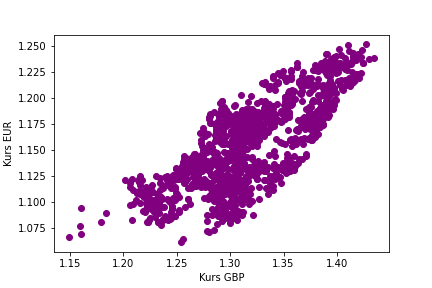
\includegraphics[scale=0.7]{XY_sc.PNG}
		\caption{Scatterplot zależności Y od X}
	\end{figure}
	\noindent Wykres pokazuje zależność danych w zbiorze Y od danych w zbiorze X. Jest to zależność liniowa. Gdy kurs EUR rośnie, rośnie też kurs GBP.
	%boxplot
	\begin{figure}[H]
		\begin{minipage}{.5\linewidth}
			\centering
			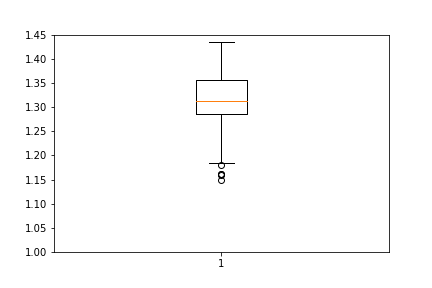
\includegraphics[scale=0.7]{X_box.PNG}
			\caption{Boxplot zbioru X}
		\end{minipage}
		$\quad$
		\begin{minipage}{.5\linewidth}
			\centering
			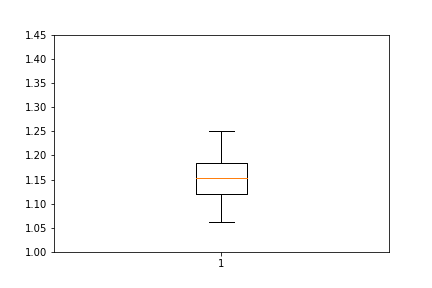
\includegraphics[scale=0.7]{Y_box.PNG}
			\caption{Boxplot zbioru Y}
		\end{minipage}
	\end{figure}
\noindent Widzimy, że zbiór X ma co najmniej 3 wartości odstające, podczas gdy Y nie ma żadnej. Mediana zbioru X jest przesunięta w stronę pierwszego kwartyla, zbioru Y wydaje się być na dokładnie pomiędzy kwartylami. Najniższa wartość X jest mocniej wysunięta niż najwyższa, podczas gdy Y są rozmieszczone w podobnej odległości od kwartyli. Żaden ze zbiorów nie ma górnej ani dolnej obserwacji ekstremalnej.
	\section{Podsumowanie}
	\noindent Zakresy, które przyjmują dane ze zbiorów X i Y nie są bardzo rozległe, dlatego nie obserwujemy ogromnych różnic przy wyliczaniu różnych statystyk, na przykład średnich. Na podstawie analizy wykresów oraz obliczeniu współczynnika korelacji odkryliśmy, że kursy walut EUR i GBP są mocno skorelowane. 
	Dane zbioru Y są bardziej skupione niż dane zbioru X, który posiada kilka wartości odstających. 
\end{document}